\documentclass[journal,compsoc]{IEEEtran}
\usepackage{tikz}
\usetikzlibrary{arrows.meta,positioning,shapes.geometric,fit,calc,backgrounds}
\usepackage{xcolor}

\definecolor{clientblue}{RGB}{235,243,250}
\definecolor{clientborder}{RGB}{50,110,180}
\definecolor{gateyellow}{RGB}{254,249,235}
\definecolor{gateborder}{RGB}{210,140,30}
\definecolor{fastpurple}{RGB}{246,240,250}
\definecolor{fastborder}{RGB}{120,60,170}
\definecolor{dbgreen}{RGB}{236,247,240}
\definecolor{dbborder}{RGB}{40,140,80}

\tikzset{
  tierbox/.style={draw=#1, fill=#1!12, rounded corners=4pt, line width=0.8pt, inner sep=3pt},
  compnode/.style={draw=#1, fill=white, rounded corners=2.5pt, line width=0.6pt, align=center, font=\scriptsize},
  arrow/.style={-{Stealth[length=2.2mm,width=1.5mm]}, line width=0.8pt, draw=black!75},
  darrow/.style={{Stealth[length=2mm]}-{Stealth[length=2mm]}, line width=0.8pt, draw=black!75},
  dasharrow/.style={-{Stealth[length=2mm]}, dashed, line width=0.7pt, draw=black!60}
}

\begin{document}

\begin{figure*}
\centering
\resizebox{0.96\textwidth}{!}{%
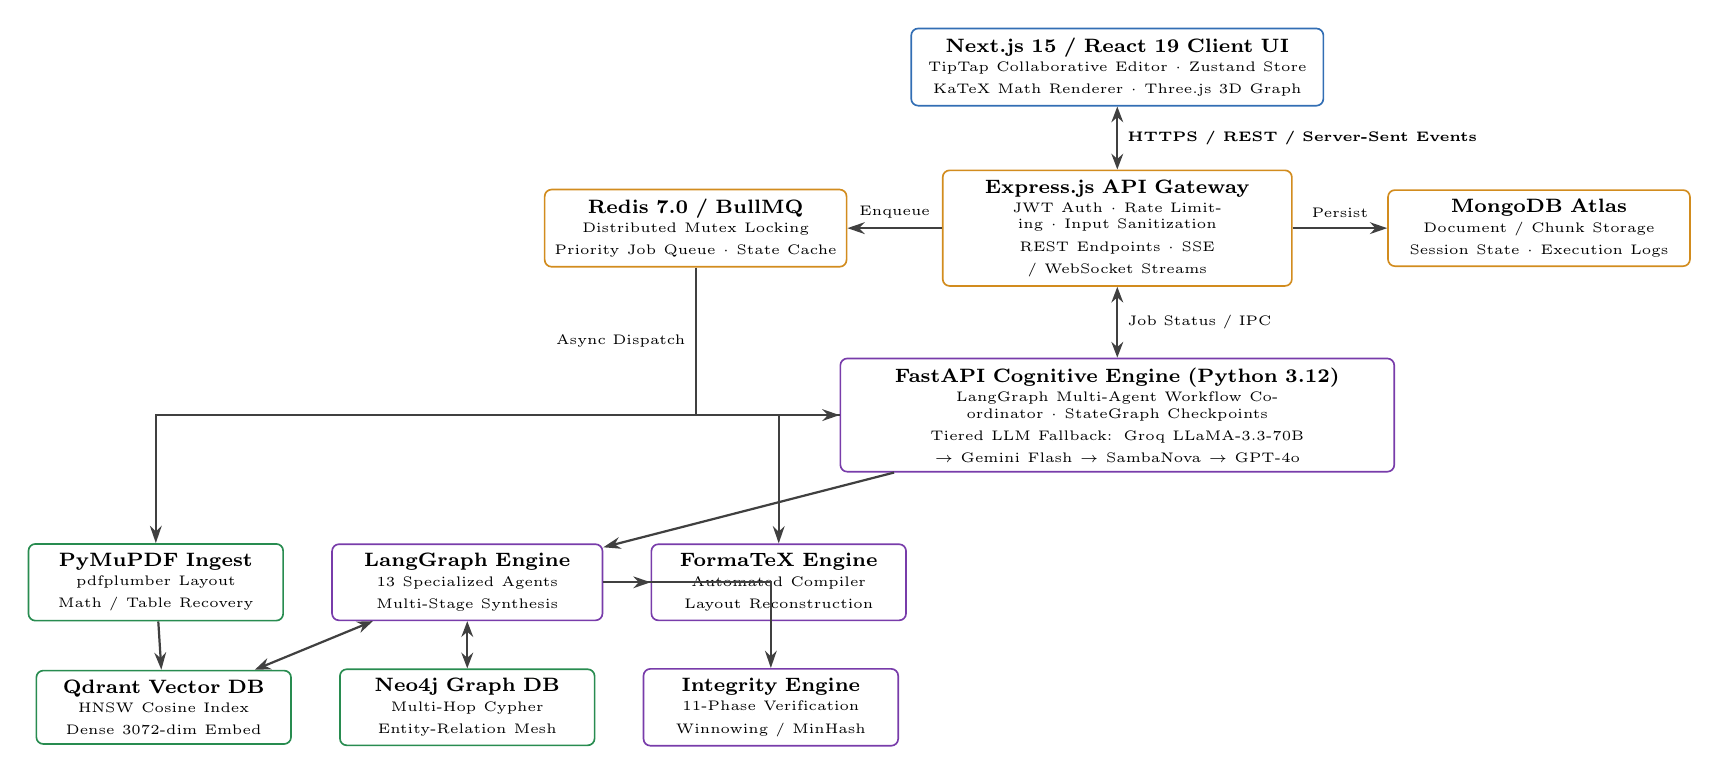
\begin{tikzpicture}[node distance=5mm and 6mm]

% --- TIER 1: Presentation & Client Tier ---
\node[compnode=clientborder, text width=50mm] (ui) {
  \textbf{Next.js 15 / React 19 Client UI}\\[1pt]
  \tiny TipTap Collaborative Editor $\cdot$ Zustand Store\\
  \tiny KaTeX Math Renderer $\cdot$ Three.js 3D Graph
};

% --- TIER 2: Gateway & Job Distribution Tier ---
\node[compnode=gateborder, text width=42mm, below=8mm of ui] (gateway) {
  \textbf{Express.js API Gateway}\\[1pt]
  \tiny JWT Auth $\cdot$ Rate Limiting $\cdot$ Input Sanitization\\
  \tiny REST Endpoints $\cdot$ SSE / WebSocket Streams
};

\node[compnode=gateborder, text width=36mm, left=12mm of gateway] (redis) {
  \textbf{Redis 7.0 / BullMQ}\\[1pt]
  \tiny Distributed Mutex Locking\\
  \tiny Priority Job Queue $\cdot$ State Cache
};

\node[compnode=gateborder, text width=36mm, right=12mm of gateway] (mongo) {
  \textbf{MongoDB Atlas}\\[1pt]
  \tiny Document / Chunk Storage\\
  \tiny Session State $\cdot$ Execution Logs
};

% --- TIER 3: Cognitive AI Orchestration Tier ---
\node[compnode=fastborder, text width=68mm, below=9mm of gateway] (fastapi) {
  \textbf{FastAPI Cognitive Engine (Python 3.12)}\\[1pt]
  \tiny LangGraph Multi-Agent Workflow Coordinator $\cdot$ StateGraph Checkpoints\\
  \tiny Tiered LLM Fallback: Groq LLaMA-3.3-70B $\to$ Gemini Flash $\to$ SambaNova $\to$ GPT-4o
};

% --- TIER 4: Agents, Processing & Storage Mesh ---
\node[compnode=fastborder, text width=32mm, below left=9mm and 30mm of fastapi] (agents) {
  \textbf{LangGraph Engine}\\[1pt]
  \tiny 13 Specialized Agents\\
  \tiny Multi-Stage Synthesis
};

\node[compnode=dbborder, text width=30mm, left=6mm of agents] (ingest) {
  \textbf{PyMuPDF Ingest}\\[1pt]
  \tiny pdfplumber Layout\\
  \tiny Math / Table Recovery
};

\node[compnode=dbborder, text width=30mm, below=6mm of agents] (neo4j) {
  \textbf{Neo4j Graph DB}\\[1pt]
  \tiny Multi-Hop Cypher\\
  \tiny Entity-Relation Mesh
};

\node[compnode=dbborder, text width=30mm, left=6mm of neo4j] (qdrant) {
  \textbf{Qdrant Vector DB}\\[1pt]
  \tiny HNSW Cosine Index\\
  \tiny Dense 3072-dim Embed
};

\node[compnode=fastborder, text width=30mm, right=6mm of agents] (formatex) {
  \textbf{FormaTeX Engine}\\[1pt]
  \tiny Automated Compiler\\
  \tiny Layout Reconstruction
};

\node[compnode=fastborder, text width=30mm, right=6mm of neo4j] (integrity) {
  \textbf{Integrity Engine}\\[1pt]
  \tiny 11-Phase Verification\\
  \tiny Winnowing / MinHash
};

% --- ARROWS ---
\draw[darrow] (ui) -- node[right, font=\tiny\bfseries] {HTTPS / REST / Server-Sent Events} (gateway);
\draw[arrow] (gateway) -- node[above, font=\tiny] {Enqueue} (redis);
\draw[arrow] (gateway) -- node[above, font=\tiny] {Persist} (mongo);
\draw[arrow] (redis) |- node[near start, left, font=\tiny] {Async Dispatch} (fastapi);
\draw[darrow] (gateway) -- node[right, font=\tiny] {Job Status / IPC} (fastapi);

\draw[arrow] (fastapi) -| (ingest);
\draw[arrow] (fastapi) -- (agents);
\draw[arrow] (fastapi) -| (formatex);

\draw[arrow] (ingest) -- (qdrant);
\draw[darrow] (agents) -- (neo4j);
\draw[darrow] (agents) -- (qdrant);
\draw[arrow] (agents) -- (formatex);
\draw[arrow] (agents) -| (integrity);

\end{tikzpicture}}
\caption{Redesigned Fig 1 Architecture}
\end{figure*}

\end{document}
